\documentclass{beamer}


\usepackage{amsmath}
\usepackage[style=alphabetic,url=true]{biblatex}
\usepackage{environ}
\usepackage{geometry}
\usepackage{graphicx}
\usepackage{tikz}
\usepackage[T2A]{fontenc}
\usepackage[utf8]{inputenc}
\usepackage{listings}


% \usetheme{Bergen}

\usecolortheme{beaver}

\setbeamertemplate{itemize item}[circle]
\setbeamertemplate{itemize subitem}{--}
\addtobeamertemplate{navigation symbols}{}{
  \usebeamerfont{footline}%
  \usebeamercolor[fg]{footline}%
  \hspace{1em}%
  \insertframenumber/\inserttotalframenumber
}
\graphicspath{ {./graphics/} }


\title{
  Bitcoin and Cryptocurrency Technologies \\
  Lecture 1: Economics and History
}

\author{Yuri Zhykin}
\date{Feb 8, 2021}

\begin{document}

\frame{\titlepage}

\begin{frame}
  \frametitle{Contacts}
  \begin{itemize}
  \item @rodentrabies on Telegram
  \item https://github.com/rodentrabies
  \end{itemize}
\end{frame}

\begin{frame}
  \frametitle{Course structure 1/2}
  \begin{itemize}
  \item History and economics of Bitcoin
    \begin{itemize}
    \item Economic concepts and properties of money
    \item Computer cryptography and cypherpunk movement
    \item Bitcoin invention and innovation
    \end{itemize}
  \item Crypto means Cryptography
    \begin{itemize}
    \item Cryptography basics
    \item Hash functions
    \item Public key cryptography
    \item Elliptic curves
    \item Cryptographic signatures
    \end{itemize}
  \item Bitcoin chain data model
    \begin{itemize}
    \item Transactions
    \item Inputs and outputs
    \item Blocks
    \item Chain of blocks and Proof of Work
    \end{itemize}
  \item[] ...
  \end{itemize}
\end{frame}

\begin{frame}
  \frametitle{Course structure 2/2}
  \begin{itemize}
  \item[] ...
  \item Bitcoin network
    \begin{itemize}
    \item Peer-to-peer network architecture
    \item Mempool and mining
    \item Network parameters and dynamics
    \end{itemize}
  \item Deep dive into Bitcoin transactions
    \begin{itemize}
    \item Transaction scripts
    \item Transaction validation
    \item Bitcoin wallets
    \end{itemize}
  \item Second layer protocols
    \begin{itemize}
    \item Scalability problem
    \item Payment channel networks
    \item Non-fungible tokens
    \end{itemize}
  \item Other cryptocurrency systems
    \begin{itemize}
    \item Ethereum: maximum flexibility
    \item Monero: maximum privacy
    \end{itemize}
  \end{itemize}
\end{frame}

\begin{frame}
  \frametitle{Economic concepts and properties of money}
  \begin{itemize}
  \item \textbf{Money is any item or verifiable record that is generally accepted as
    payment for goods and services}
  \item \textbf{Durable} - able to retain its value over time
  \item \textbf{Portable} - easy to transport in sufficiently large quantities
  \item \textbf{Divisible} - can be divided into smaller quantities to represent whole
    range of value
  \item \textbf{Fungible} - two units of the same nominal value must be equally valuable
  \item \textbf{Scarce} - it must be very hard to increase the supply
  \item \textbf{Recognizable} - it must be easy to find peers willing to accept
    it as payment
  \end{itemize}
\end{frame}

\begin{frame}
  \frametitle{Money before Bitcoin}
  \begin{itemize}
  \item Seashells
  \item Silver
  \item Gold
  \item Paper money
  \item Fiat money
  \end{itemize}
\end{frame}

\begin{frame}
  \frametitle{Cryptography and electronic money}
  \begin{itemize}
  \item \textbf{Cryptography} is a method of protecting information and
    communications through the use of secrets that prevent third parties from
    accessing it
  \item Traditional electronic money - encrypted and centrally managed ledgers
  \item Is it possible to eliminate central management?
  \item \textbf{Byzantine Generals Problem} - how can two generals agree on when
    to attack, when then don't trust each other?
  \item \textbf{How can multiple parties come to a consensus when they trust no
      one?}
  \end{itemize}
\end{frame}

\begin{frame}
  \frametitle{Centralized monetary system}
  \begin{itemize}
  \item In most cases government is the central entity controlling monetary
    supply
  \item Assumption that government is competent enough to ``manage'' the economy
  \item Government can inflate fiat currency, effectively extracting resources
    from \textbf{all} its people without their consent
  \item Exclusive control over money is the ultimate tool of controlling people
    for totalitarian regimes
  \end{itemize}
\end{frame}

\begin{frame}
  \frametitle{Cypherpunk movement}
  \begin{itemize}
  \item Widespread use of strong cryptography and privacy-enhancing technologies
    as a route to social and political change
  \item \textbf{Can we use strong cryptography to solve BGP and create a
      decentralized monetary system?}
  \item Several attempts:
    \begin{itemize}
    \item David Chaum - DigiCash, 1989
    \item Wei Dai - b-money, 1998
    \item Nick Szabo - Bit Gold, 1998
    \item Adam Back - Hashcash, 1997-2002
    \end{itemize}
  \end{itemize}
\end{frame}

\begin{frame}
  \frametitle{Satoshi Nakamoto and Bitcoin Genesis 1/3}
  \begin{itemize}
  \item Financial crisis of 2007-2008
  \item On October 31, 2008, pseudonymous person \textbf{Satoshi Nakamoto}
    published a whitepaper titled "Bitcoin: A Peer-to-Peer Electronic Cash
    System"
  \item In late 2008 - early 2009, Nakamoto contacted Wei Dai, Adam Back and Hal
    Finney about the electronic cash system he was working on
  \item On January 9, 2009, Nakamoto released version 0.1 of the Bitcoin
    software and launched the network by mining the \textbf{genesis block}
  \end{itemize}
\end{frame}

\begin{frame}[fragile]
  \frametitle{Satoshi Nakamoto and Bitcoin Genesis 2/3}
  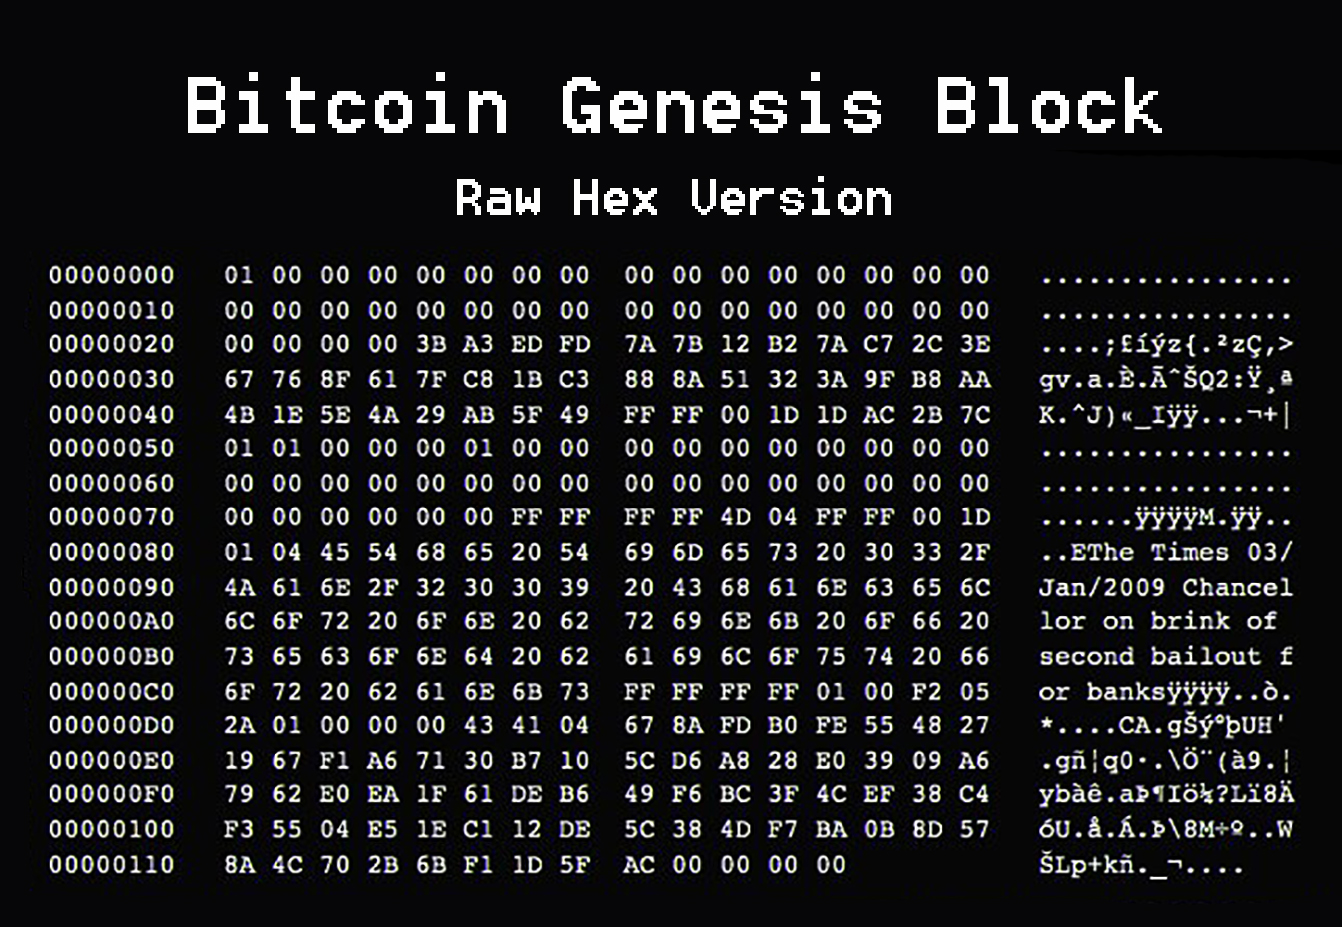
\includegraphics[width=\textwidth]{genesis-block}
\end{frame}

\begin{frame}
  \frametitle{Satoshi Nakamoto and Bitcoin Genesis 3/3}
  \begin{itemize}
  \item Satoshi Nakamoto continued Bitcoin development until mid-2010, when he
    transferred control over the repository to Gavin Andersen
  \item On April 26, 2011, Nakamoto wrote his last known email to Gavin
    Andersen, and never appeared online since
  \item The Bitcoin software written by Satoshi Nakamoto is the basis for the
    Bitcoin Core project (https://github.com/bitcoin/bitcoin)
  \end{itemize}
\end{frame}

\begin{frame}
  \frametitle{Bitcoin invention}
  \begin{itemize}
  \item Cryptographic Proof of Work system solves the generalized Byzantine
    Generals Problem, eliminating the need to trust anyone on the network
  \item \textbf{Bitcoin is decentralized money}
  \item Transaction scripting system provides flexibility for more complex use
    cases then simple value transfering
  \item \textbf{Bitcoin is programmable money}
  \end{itemize}
\end{frame}

\begin{frame}
  \frametitle{Market acceptance}
  \begin{itemize}
  \item In 2010, the first known commercial transaction using bitcoin occurred
    when programmer Laszlo Hanyecz bought two Papa John's pizzas for 10,000 BTC
  \item In 2011, Bitcoin becomes accepted as donations by Electronic Frontier
    Foundation and WikiLeaks
  \item In 2011, price went from \$0.30 to \$5.27
  \item In 2012, from \$5.25 to \$13.30
  \item In 2013, from \$13.30 to \$770
  \item On February 8, 2021, bitcoin price is \$38831.60
  \end{itemize}
\end{frame}

\begin{frame}
  \frametitle{Additional resources}
  \begin{itemize}
  \item https://www.activism.net/cypherpunk/manifesto.html - Cypherpunk Manifesto
  \item https://unenumerated.blogspot.com - Nick Szabo's Blog
  \item The Bitcoin Standard: The Decentralized Alternative to Central Banking,
    2018 - Saifedean Ammous
  \item Human Action: A Treatise on Economics, 1949 - Ludwig von Mises
  \end{itemize}
\end{frame}

\begin{frame}
  \frametitle{The end}
  \begin{center}
    Thank you!
  \end{center}
\end{frame}

\end{document}

%%% Local Variables:
%%% mode: latex
%%% TeX-master: t
%%% End:
